\chapter{پیاده سازی و نتایج}

\section{پیاده سازی پلتفرم}
\subsection{سیستم مدیریت}

در پلتفرم‌های بزرگ، نیاز به سیستمی برای مدیریت پلتفرم به وضوح احساس می‌شود. این سیستم باید قابلیت هماهنگی و یکپارچگی بین اجزای مختلف را داشته باشد تا اطمینان حاصل شود که همه بخش‌ها به درستی و بدون مشکل عمل می‌کنند. ویژگی‌های حیاتی این سیستم شامل استفاده از ابزارهای خودکارسازی و نظارت پیشرفته، مدیریت بهینه منابع سخت افزاری، پیاده‌سازی فرآیندهای مستمر بهبود و به‌روزرسانی، مدیریت دسترسی‌ها و امنیت و مستندسازی فرآیندها و تغییرات است. سیستم مدیریت شامل تمامی ابزارهای مدیریتی مانند مدیریت مخازن مولفه‌ها، کد و خط لوله \lr{CI/CD}، مانیتورینگ کل سیستم و جمع آوری لاگ است. علاوه بر این، استراتژی استقرار پروژه، اعمال مهاجرت‌ها\footnote{\lr{Migrations}}، پیکربندی پروژه‌ها، مدیریت سرورهای \lr{DNS} و \lr{NTP}\footnote{\lr{Network Time Protocol}} و استفاده از ابزارهایی مانند \lr{Foreman} برای نصب سیستم‌عامل به صورت \lr{PXE} نیز توسط همین سیستم مدیریت می‌شود.

به منظور پیاده سازی این سیستم، ما دو ماشین مجزا برای مدیریت پلتفرم به منظور ایجاد قابلیت تحمل خطا\footnote{\lr{Fault Tolerance}} و دسترسی پذیری بالا\footnote{\lr{High Availability}}  قرار می‌دهیم. از آنجایی که فرآیند و پروسه سنگینی روی این ماشین ها انجام نمی شود مشخصات کمتری می تواند به نسبت ماشین های پروژه داشته باشد. مشخصات سخت افزاری هرکدام از این ماشین ها در جدول
~\ref{tb: management conf}
قرار دارد.  این ماشین ها به صورت ماشین مجازی با استفاده از \lr{OpenStack} ساخته می شود. ماشین‌های مدیریت باید برای نصب و راه‌اندازی ابزارهای مدیریت پلتفرم پیکربندی شوند و این کار با استفاده از ابزار \lr{Ansible} انجام می گیرد. به این منظور \lr{Role} های مشخصی برای هر بخش نوشته شده است تا بتوان بدون هیچ کار دستی و به صورت کاملا خودکار سیستم ها را پیکربندی کرد. این \lr{Role} های انسیبلی با استفاده از قاعده نسخه گذاری \lr{Semantic} نسخه گذاری شده و در مخزن \lr{raw} موجود در \lr{Nexus} که یک ابزار مدیریت مخازن مولفه می باشد نگه داری خواهند شد. در نهایت برای پیکربندی سیستم، \lr{Role} موردنظر با نسخه مشخص از \lr{Nexus} گرفته شده و بااستفاده از \lr{Ansible} ماشین ها پیکربندی می شوند. از آنجایی که این پیکربندی در محیط های مختلف مانند توسعه و عملیات می تواند متفاوت باشد، ما با استفاده از قابلیت \lr{Overriding} در این ابزار مقادیر پیش فرض را برای هر محیط تغییر خواهیم داد. به همین منظور اسکریپتی طراحی شده که در لینک 
گیت هاب\footnote{\url{https://github.com/abolfazlyarian/mlops.git}} قابل مشاهده است.

\begin{table}
	\centering
	\caption{مشخصات سخت افزاری ماشین های مدیریت}
	\label{tb: management conf}
	\begin{tabular}{|c|c|c|c|}
		\hline
		\lr{OS} & \lr{Storage} &  \lr{RAM} & \lr{CPU} \\ \hline
		\lr{Ubuntu 18.04} & \lr{512 GB} & \lr{8 GB} & \lr{4 Core} \\ \hline
	\end{tabular}
\end{table}

پروسه پیکربندی و نصب ابزار در ماشین های مدیریت به صورت زیر انجام می گردد:
\begin{enumerate}
	\item 
	پیکربندی ماشین ها:
این قسمت شامل نصب و پیکربندی ابزارهایی نظیر
\lr{BIND}
برای سرور \lr{DNS}،
\lr{APT}
برای مدیریت ابزار در سیستم عامل \lr{Ubuntu}،
\lr{pip}
برای مدیریت کتابخانه ها پایتون،
\lr{chrony}
برای سرور \lr{NTP}
،\lr{LDAP} 
برای مدیریت کاربران و … می باشد.
	\item
نصب و پیکربندی \lr{Docker}: از آنجایی که مدیریت ابزارها به صورت کانتینر مناسب تر است، برای انجام مراحل بعدی نیاز به نصب \lr{Docker} می باشد. پس از نصب به منظور ذخیره سازی تمام مولفه ها مورد استفاده به مخزن ساخته شده در \lr{Nexus} مدیریت متصل خواهد شد.
	\item 
 \lr{Nexus}: از این ابزار به منظور مدیریت مخازن مولفه ها استفاده شده است. مخازن مورد استفاده ما \lr{APT}، 
	\lr{pip}،
	\lr{Docker}
	و \lr{raw} می باشد (شکل 
	~\ref{fig: nexus repo}).

	\item 
 \lr{Jenkins}: از این ابزار به منظور اجرا و مدیریت خط لوله های \lr{CI/CD} پروژها و هم چنین پیکربندی آن ها توسط مدیران سیستم استفاده می شود (شکل 
	~\ref{fig: jenkins}).
	
	\item 
 \lr{GitLab}: به منظور مدیریت کد در پروژه ها و هم چنین مدیریت \lr{Role}های انسیبلی برای پیکربندی پروژها استفاده می شود (شکل 
	~\ref{fig: gitlab}).
	
\begin{figure}[!t]
	\centering
	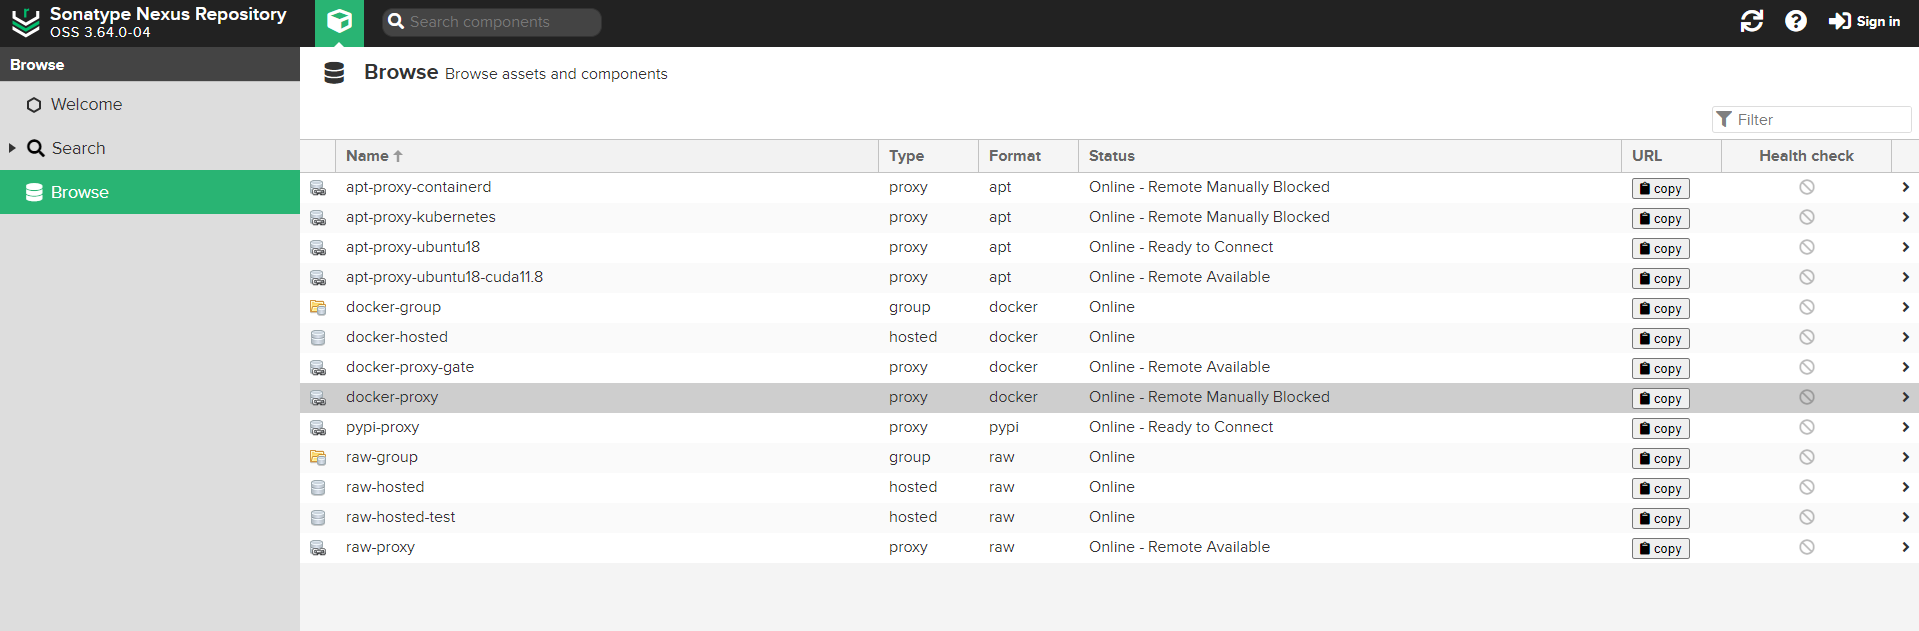
\includegraphics[scale=0.3]{nexus-repo.png}
	\caption{مخازن مولفه در \lr{Nexus}}
	\label{fig: nexus repo}
\end{figure}
\begin{figure}[!t]
	\centering
	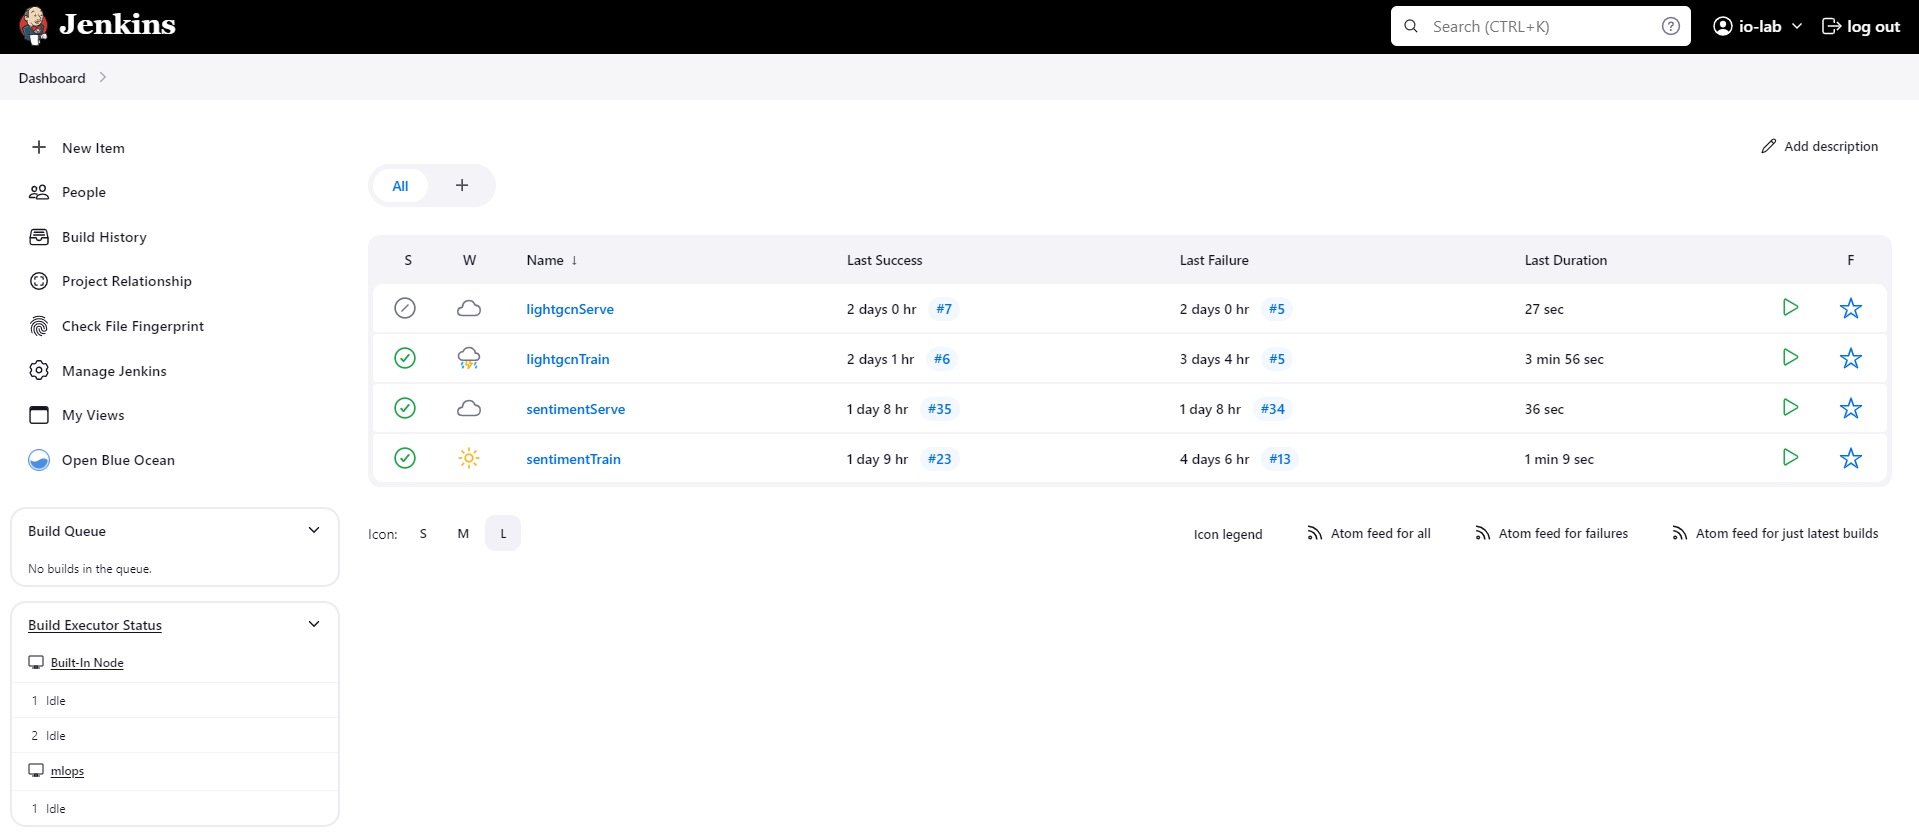
\includegraphics[scale=0.3]{jenkins1.png}
	\caption{خط لوله ها \lr{CI/CD} در \lr{Jenkins}}
	\label{fig: jenkins}
\end{figure}
\begin{figure}[!t]
	\centering
	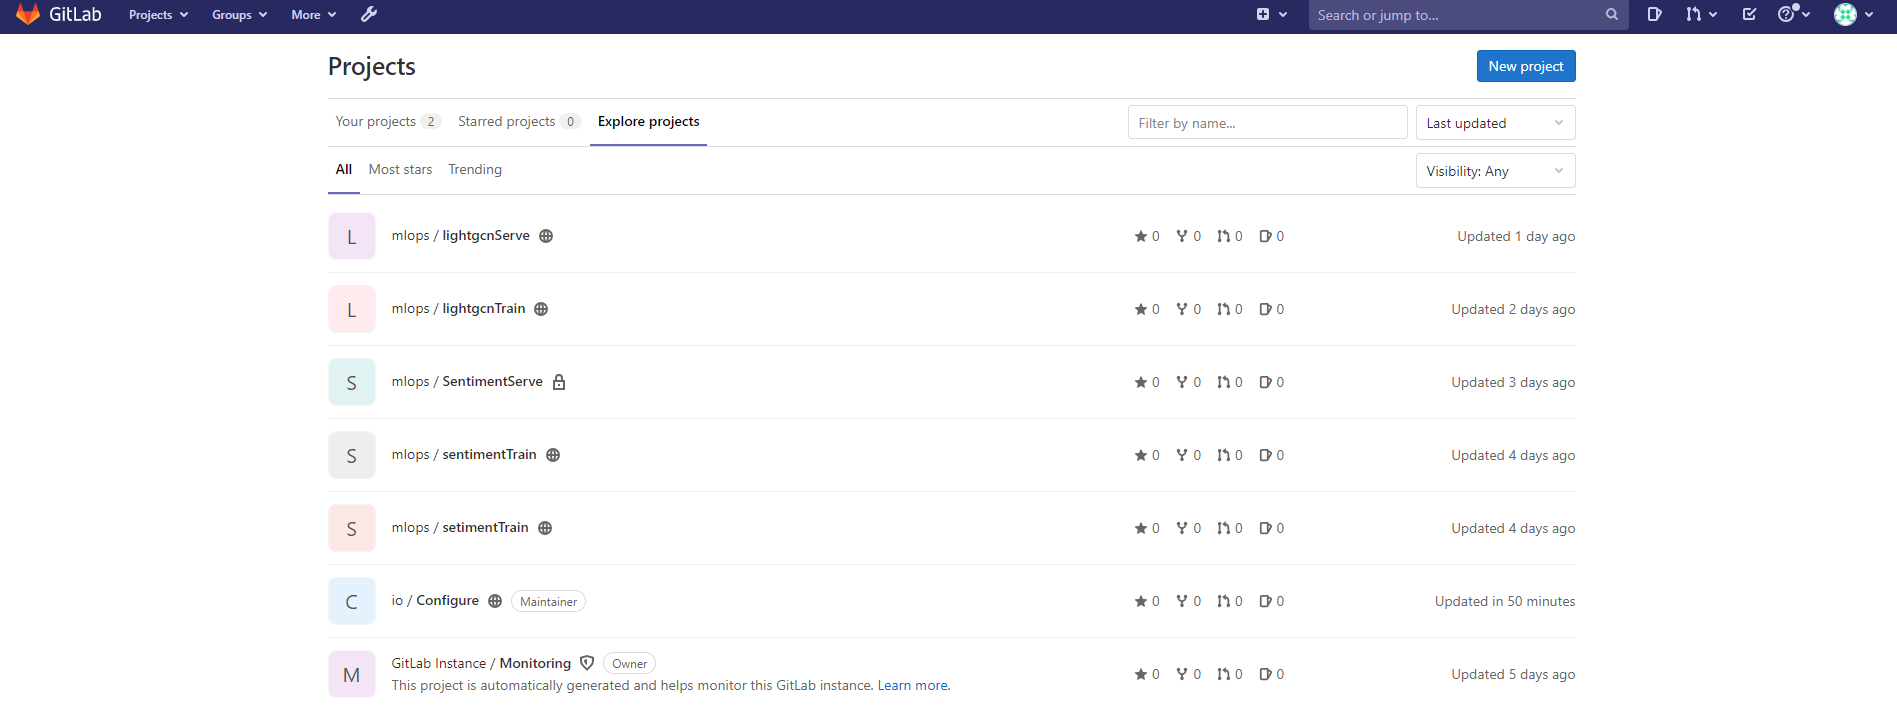
\includegraphics[scale=0.3]{gitlab.png}
	\caption{مخازن کد در \lr{Gitlab}}
	\label{fig: gitlab}
\end{figure}
\end{enumerate}
\clearpage
\subsection{خوشه کوبرنتیز}
در طراحی یک پلتفرم \lr{MLOps} جامع و کارآمد که تمامی ابزارهای مورد نیاز را در بر می‌گیرد، هدف اصلی ایجاد یک بستر یکپارچه، مقیاس‌پذیر و انعطاف‌پذیر برای مدیریت چرخه حیات مدل‌های یادگیری ماشین است. این پلتفرم شامل مجموعه‌ای از ابزارها و تکنولوژی‌های متن‌باز است که همگی روی خوشه کوبرنتیز مستقر می‌شوند. استفاده از کوبرنتیز در پلتفرم‌های \lr{MLOps} به دلیل قابلیت‌های منحصر به فرد آن در مدیریت خودکار، مقیاس‌پذیری و کارایی منابع است. 

برای نصب خوشه کوبرنتیز و انجام تست های اولیه پروژه \lr{MLOps}
، 4 ماشین مجازی با مشخصات ذکر شده در جدول 
~\ref{tb: mlops conf}
 استفاده شده است. در این پیاده سازی سه ماشین اول به عنوان گره اصلی و ماشین چهارم به عنوان گره کاری انتخاب شده است. همانند سیستم های مدیریت، ابتدا ماشین های مجازی که توسط \lr{OpenStack} ساخته خواهند شد پیکربندی می شوند. پس از آن با استفاده از ابزار \lr{Kubeadm} خوشه کوبرنتیز پیاده سازی خواهد شد.
\begin{table}
	\centering
	\caption{مشخصات سخت افزاری ماشین های خوشه کوبرنتیز}
	\label{tb: mlops conf}
	\begin{tabular}{|c|c|c|c|}
		\hline
		\lr{OS} & \lr{Storage} &  \lr{RAM} & \lr{CPU} \\ \hline
		\lr{Ubuntu 18.04} & \lr{2 TB} & \lr{128 GB} & \lr{40 Core} \\ \hline
	\end{tabular}
\end{table}

\subsubsection{پیاده سازی خوشه کوبرنتیز}
برای نصب و پیاده‌سازی کوبرنتیز با استفاده از \lr{kubeadm}، ابتدا پیش‌نیازهایی مانند \lr{Containerd} و بسته‌های کوبرنتیز شامل \lr{kubeadm}، \lr{kubelet} و \lr{kubectl} آماده می‌شوند. پس از پیکربندی سیستم و نصب \lr{Containerd}، بسته‌های مورد نیاز نصب شده و \lr{Swap} غیرفعال می‌گردد، چرا که کوبرنتیز برای عملکرد بهینه نیاز به غیرفعال بودن \lr{Swap} دارد. راه‌اندازی خوشه با اجرای دستور \lr{kubeadm init} بر روی گره اصلی آغاز می‌گردد. این دستور تنظیمات اولیه را انجام داده و فایل پیکربندی برای \lr{kubectl} ایجاد می‌کند که باید برای دسترسی به خوشه تنظیم گردد. پس از آن، نصب رابط شبکه کانتینر\footnote{\lr{Container Network Interface (CNI)}} انجام می‌شود و در این مورد، ابزار \lr{Calico} مورد استفاده قرار می‌گیرد. نصب \lr{Calico} امکان برقراری ارتباط بین پادها در داخل خوشه را فراهم می‌سازد.

در مرحله بعد، گره های کارگر به خوشه اضافه می‌شوند. دستورات لازم برای پیوستن نودهای کارگر به خوشه که از دستور قبل به‌دست آمده‌اند، بر روی هر گره کارگر اجرا می‌گردد تا این گره ها به گره اصلی متصل شوند. در نهایت، وضعیت گره ها و صحت پیوستن آن‌ها به خوشه با استفاده از \lr{kubectl get nodes} بررسی می‌گردد و اطمینان حاصل می‌شود که همه گره ها به درستی اضافه شده و آماده به کار هستند. این روش نصب، راهی سریع و مؤثر برای راه‌اندازی خوشه کوبرنتیز فراهم می‌آورد که امکان اضافه کردن گره  های جدید و مدیریت بهتر و مقیاس‌پذیری را به سهولت فراهم می‌سازد. تمامی این فرآیند با استفاده از \lr{Role} های انسیبلی روی ماشین های پروژه انچام می گردد.

\subsubsection{پیاده سازی مولفه های پروژه}
تمامی مولفه ها انتخاب شده در طراحی معماری فصل قبل با استفاده از \lr{Helm} که وظیفه مدیریت مولفه ها را دارد انجام می گیرد. \lr{Helm} یک ابزار قدرتمند برای مدیریت بسته‌های نرم‌افزاری کوبرنتیز است که فرآیند استقرار، بروزرسانی و مدیریت برنامه‌ها را ساده‌تر می‌کند. نصب یک چارت با استفاده از \lr{Helm} این امکان را می‌دهد که برنامه‌ها و سرویس‌ها با کمترین تلاش ممکن و به صورت اتوماتیک در خوشه کوبرنتیز مستقر شوند. چارت مورد نظر با استفاده از دستور \lr{helm install} به راحتی نصب می‌گردد. این دستور، چارت مورد نظر را از مخازن موجود در \lr{Nexus} دانلود کرده و آن را در خوشه کوبرنتیز مستقر می‌کند. این کار نیز با استفاده از یک \lr{Role} انسیبلی که نوشته شده است انجام می گیرد. 

یکی از مزایای استفاده از \lr{Helm}، قابلیت تنظیم پارامترهای چارت‌ها در زمان نصب است. این قابلیت امکان سفارشی‌سازی چارت‌ها را براساس نیازهای خاص پروژه فراهم می‌کند. با استفاده از این ویژگی و قابلیت مشابه در انسیبل، همانند قبل برای هر محیط مقادیر خاص آن محیط را پیکربندی می کنیم. علاوه بر این، \lr{Helm} با ارائه قابلیت بازگشت پذیری، امکان بازگشت به نسخه‌های قبلی چارت‌ها را نیز فراهم می‌سازد که این ویژگی برای مدیریت نسخه‌ها و رفع مشکلات بسیار مفید است. 

تمامی مولفه های اصلی نصب شده روی خوشه کوبرنتیز به منظور پیاده سازی پلتفرم \lr{MLOps} در شکل
??????????????
 نشان داده شده است. نکته ای که راجع به این مولفه ها لازم به ذکر است، به منظور افزایش قابلیت اطمینان و تحمل خطا، استفاده بیش از یک \lr{replica} برای هر مولفه ضروری است. این امر باعث می‌شود تا در صورت خرابی یکی از نمونه‌ها، مولفه مربوطه به کار خود ادامه دهد و سرویس‌دهی دچار اختلال نشود.
در شکل 
~\ref{fig: resource use no load}
نیز میزان مصرف منابع سخت افزاری سیستم زمانی که پلتفرم زیر بار نیست نشان داده شده است. همان طور که می بینید میزان مصرف منابع سخت افزاری به صورت یکنواخت به خوبی توزیع شده است که منجر به استفاده بهینه از منابع سخت افزاری می گردد.

\begin{figure}[!b]
	\centering
	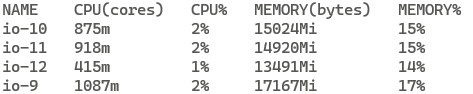
\includegraphics[scale=0.7]{resource-use1.png}
	\caption{میزان مصرف منابع سخت افزاری پلتفرم بدون بار}
	\label{fig: resource use no load}
\end{figure}
\clearpage
\section{حل مسئله و نتایج}


